\documentclass[14pt]{extreport}
\usepackage{cmap}
\usepackage[utf8]{inputenc}
\usepackage[english,ukrainian]{babel}
\usepackage{graphicx}
\usepackage{geometry}
\usepackage{listings}
\usepackage{amsmath}
\usepackage{float}
\geometry{
	a4paper,
	left=20mm,
	right=20mm,
	top=20mm,
	bottom=20mm
}
\lstset{
	language=bash,
	tabsize=4,
	breaklines,
	keepspaces,
	showstringspaces=false,
}
\graphicspath{ {./pictures} }
\setlength{\parindent}{4em}

\newcommand\subject{Бази даних}
\newcommand\lecturer{асистент кафедри ПЗ\\Білоіваненко М.В.}
\newcommand\teacher{асистент кафедри ПЗ\\Білоіваненко М.В.}
\newcommand\mygroup{ПЗ-32}
\newcommand\lab{5}
\newcommand\theme{Розробка запитів, що виконують вибірку із декількох таблиць предметної області}
\newcommand\purpose{Розробити запити, що виконують вибірку із декількох таблиць предметної області}

\begin{document}
\begin{normalsize}
	\begin{titlepage}
		\thispagestyle{empty}
		\begin{center}
			\textbf{МІНІСТЕРСТВО ОСВІТИ І НАУКИ УКРАЇНИ\\
				НАЦІОНАЛЬНИЙ УНІВЕРСИТЕТ "ЛЬВІВСЬКА ПОЛІТЕХНІКА"}
		\end{center}
		\begin{flushright}
			Інститут \textbf{КНІТ}\\
			Кафедра \textbf{ПЗ}
		\end{flushright}
		\vspace{200pt}
		\begin{center}
			\textbf{ЗВІТ}\\
			\vspace{10pt}
			До лабораторної роботи № \lab\\
			\textbf{На тему}: “\textit{\theme}”\\
			\textbf{З дисципліни}: “\subject”
		\end{center}
		\vspace{40pt}
		\begin{flushright}
			
			\textbf{Лектор}:\\
			\lecturer\\
			\vspace{10pt}
			\textbf{Виконав}:\\
			
			студент групи \mygroup\\
			Коваленко Д.М.\\
			\vspace{10pt}
			\textbf{Прийняв}:\\
			
			\teacher\\
			
			\vspace{28pt}
			«\rule{1cm}{0.15mm}» \rule{1.5cm}{0.15mm} 2023 р.\\
			$\sum$ = \rule{1cm}{0.15mm}……………\\
			
		\end{flushright}
		\vspace{\fill}
		\begin{center}
			\textbf{Львів — 2023}
		\end{center}
	\end{titlepage}
		
	\begin{description}
		\item[Тема.] \theme.
		\item[Мета.] \purpose.
	\end{description}

	\section*{Лабораторне завдання}
	Розробити не менше 5 запитів, що виконують вибірку із декількох таблиць предметної області. Врахувати актуальність, форму представлення та можливі фільтри. Опис змісту запитів та корисні вхідні умови зафіксувати текстом. Деякі запити зберегти як представлення (VIEW).
	
	Запити повинні використовувати: декілька операторів порівняння, базові функції обробки дати, рядків, групування, агрегатні функції, сортування, обмеження кількості.
	
	\section*{Хід роботи}
	Запит, що отримує назву кожного маршруту та назви зупинок, що належать цьому маршруту у вигляді списку.
	
	Запит збережений як представлення (VIEW), що дозволяє  вибирати лише певні маршрути.
	
	\iffalse
	\begin{lstlisting}
		create view stops as
		select rs.route_id, s.name, s.lon, s.lat, rs.ord_index
		from route_stop rs
		join stop s on rs.stop_id = s.id
		order by rs.route_id, rs.ord_index;
		
		select r.name, array_agg(s.name) as stops
		from stops s
		join route r on s.route_id = r.id
		group by r.name
		order by r.name;
	\end{lstlisting}
	\fi
	
	\begin{figure}[H]
		\centering
		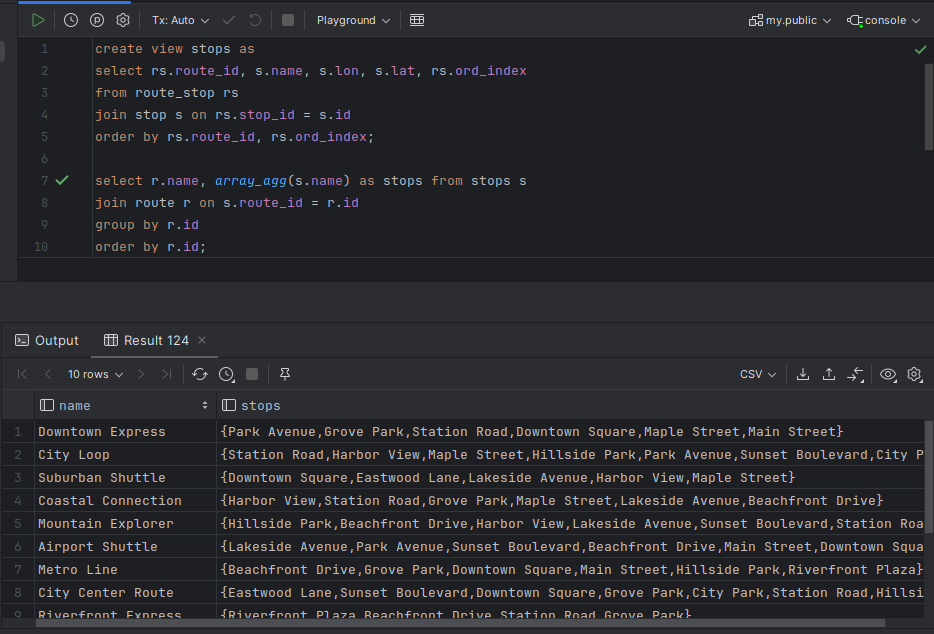
\includegraphics[scale=0.5]{1}
		\caption{Код та результат виконання запиту}
	\end{figure}
	
	Запит, що отримує номерний знак та прибуток 5-ти найприбутковіших транспортних засобів що обраховується за різницею між загальною вартістю квитків придбаних у цьому транспортному засобі та витратами на його утримання за останні 30 днів .
	
	\iffalse
	\begin{lstlisting}[language=sql]
create view last_spending as
select v.license_plate,
	max(vm.time) as last_time,
	sum(vm.cost_total) as total
from vehicle_maintenance vm
join vehicle v on vm.vehicle_id = v.id
where now() - vm.time < interval '30 days'
group by v.license_plate;

create view last_income as
select v.license_plate, sum(fare) as total
from ticket t
join vehicle v on t.vehicle_id = v.id
where now() - t.time < interval '30 days'
group by v.license_plate;

select ls.license_plate, li.total - ls.total as total
from last_spending ls
join last_income li on ls.license_plate = li.license_plate
order by total desc
limit 5;
	\end{lstlisting}
	\fi
	\begin{figure}[H]
		\centering
		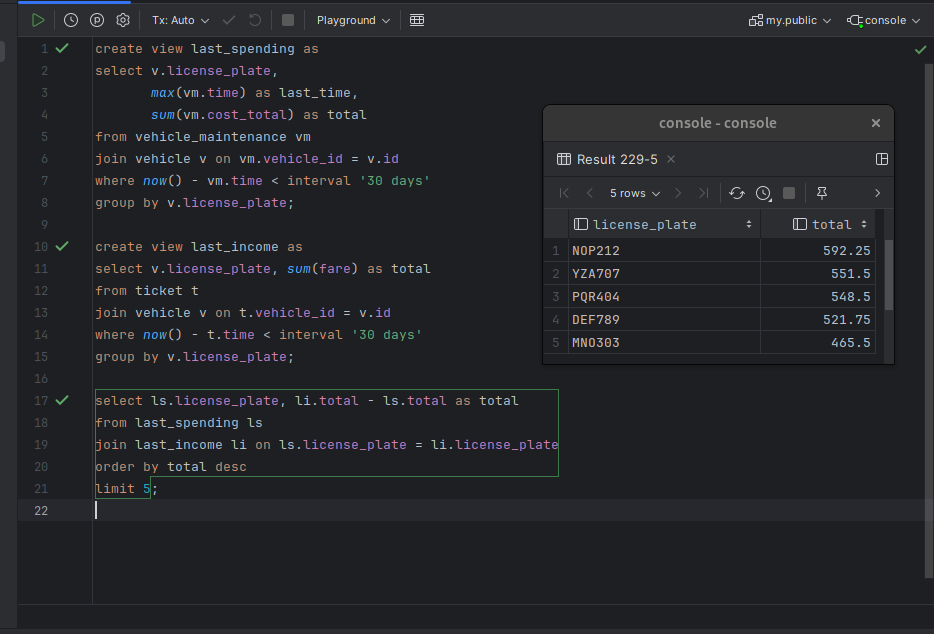
\includegraphics[scale=0.5]{2}
		\caption{Код та результат виконання запиту}
	\end{figure}
	\pagebreak
	Запит, що повертає назви маршрутів, що містять дві вказані зупинки.
	
	\iffalse
	\begin{lstlisting}[language=sql]
	create view stops as
	select
		s1.name as from_stop,
		s2.name as to_stop,
		r.name as routes
	from stop s1
	cross join stop s2
	join route_stop rs1 on rs1.stop_id = s1.id
	join route_stop rs2 on rs2.stop_id = s2.id
	join route r on rs1.route_id = rs2.route_id and rs1.route_id = r.id
	where s1.id <> s2.id;
	
	select routes
	from stops
	where from_stop = 'Beachfront Drive' and to_stop = 'Lakeside Avenue';
	\end{lstlisting}
	\fi
	\begin{figure}[H]
		\centering
		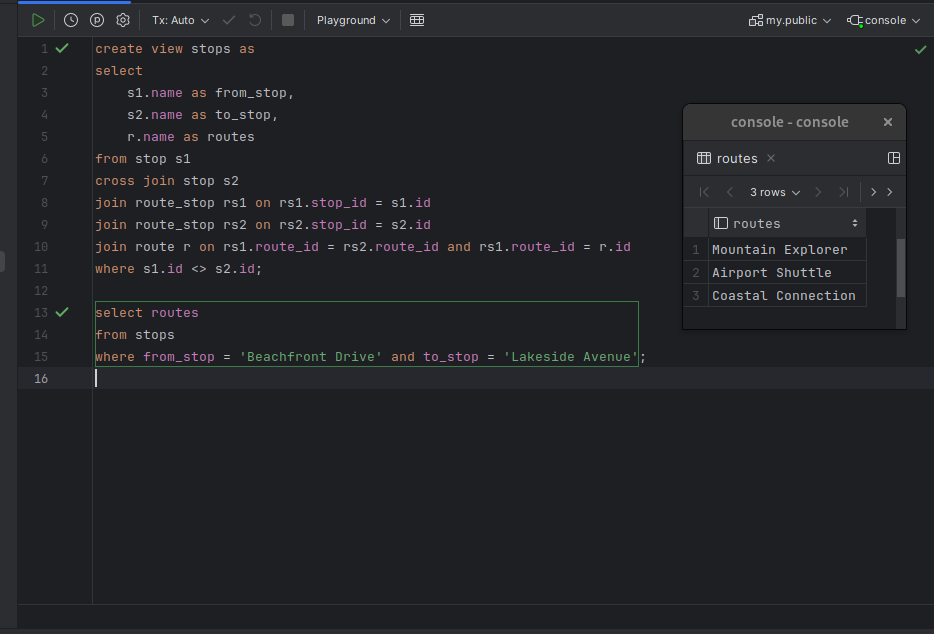
\includegraphics[scale=0.5]{3}
		\caption{Код та результат виконання запиту}
	\end{figure}
	\pagebreak
	Запит, що повертає назву початкової та кінцевої зупинки, номерний знак транспортного засобу та час у хвилинах через який він прибуває на початкову зупинку використовуючи view з попереднього запиту.
	
	\iffalse
	\begin{lstlisting}[language=sql]
		create view stops as
		select
			s1.name as from_stop,
			s2.name as to_stop,
			r.id as routes
		from stop s1
		cross join stop s2
		join route_stop rs1 on rs1.stop_id = s1.id
		join route_stop rs2 on rs2.stop_id = s2.id
		join route r on rs1.route_id = rs2.route_id and rs1.route_id = r.id
		where s1.id <> s2.id;
		
		select
			s.from_stop,
			s.to_stop,
			v.license_plate,
			floor(extract(epoch from sch.arrival_time - now()) / 60) as arrival_in_minutes
		from route_vehicle rv
		cross join stops s
		join schedule sch on s.routes = sch.route_id
		join vehicle v on rv.vehicle_id = v.id
		where s.from_stop = 'Beachfront Drive'
			and s.to_stop = 'Lakeside Avenue'
			and rv.route_id = s.routes
		order by arrival_in_minutes
	\end{lstlisting}
	\fi
	\begin{figure}[H]
		\centering
		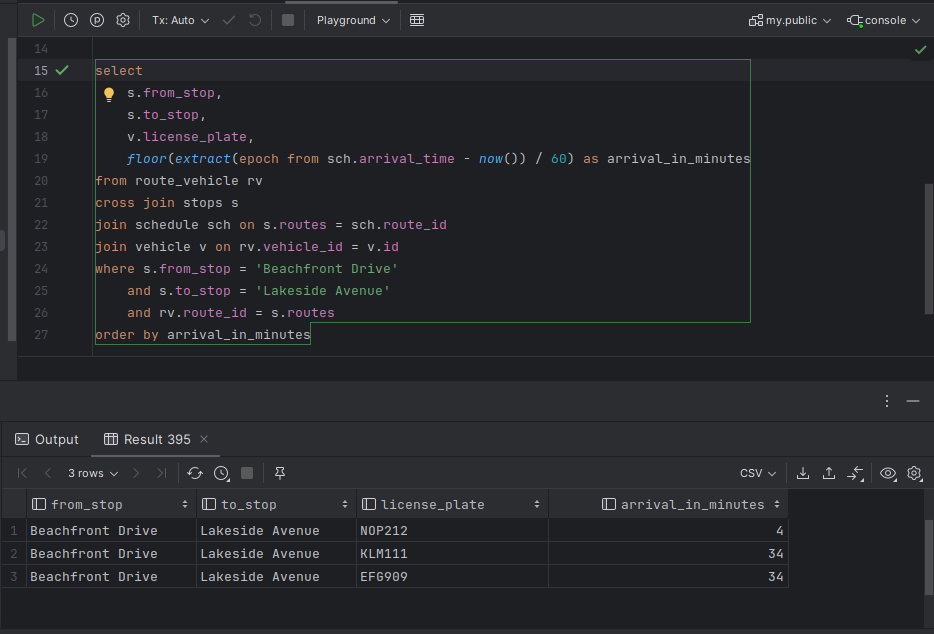
\includegraphics[scale=0.5]{4}
		\caption{Код та результат виконання запиту}
	\end{figure}
	\pagebreak
	Запит, що повертає текст повідомлення, емайл та ім'я користувача та час створення відгуків за останні 30 днів, що ймовірно є негативними адже містять у собі такі слова як `need`, `crash`, `slow`, `could be`, `bad`.
	
	\iffalse
	\begin{lstlisting}
		select message, email, name, time from feedback
		where message ilike '%need%'
			or message ilike '%crash%'
			or message ilike '%slow%'
			or message ilike '%could be%'
			or message ilike '%bad%'
			and now() - time < interval '30 days'
		order by time desc
	\end{lstlisting}
	\fi
	\begin{figure}[H]
		\centering
		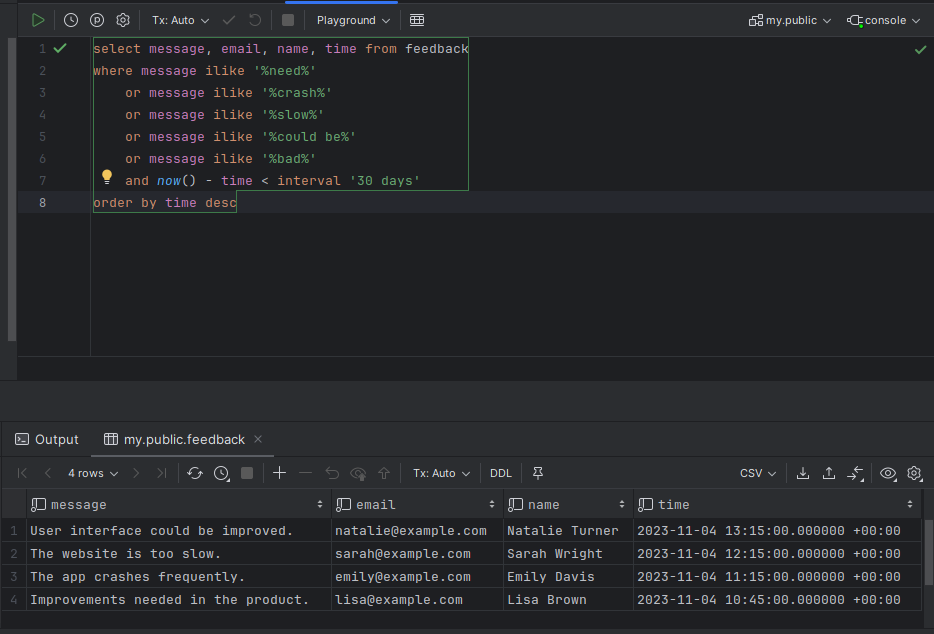
\includegraphics[scale=0.5]{5}
		\caption{Код та результат виконання запиту}
	\end{figure}
	
	\begin{figure}[H]
		\centering
		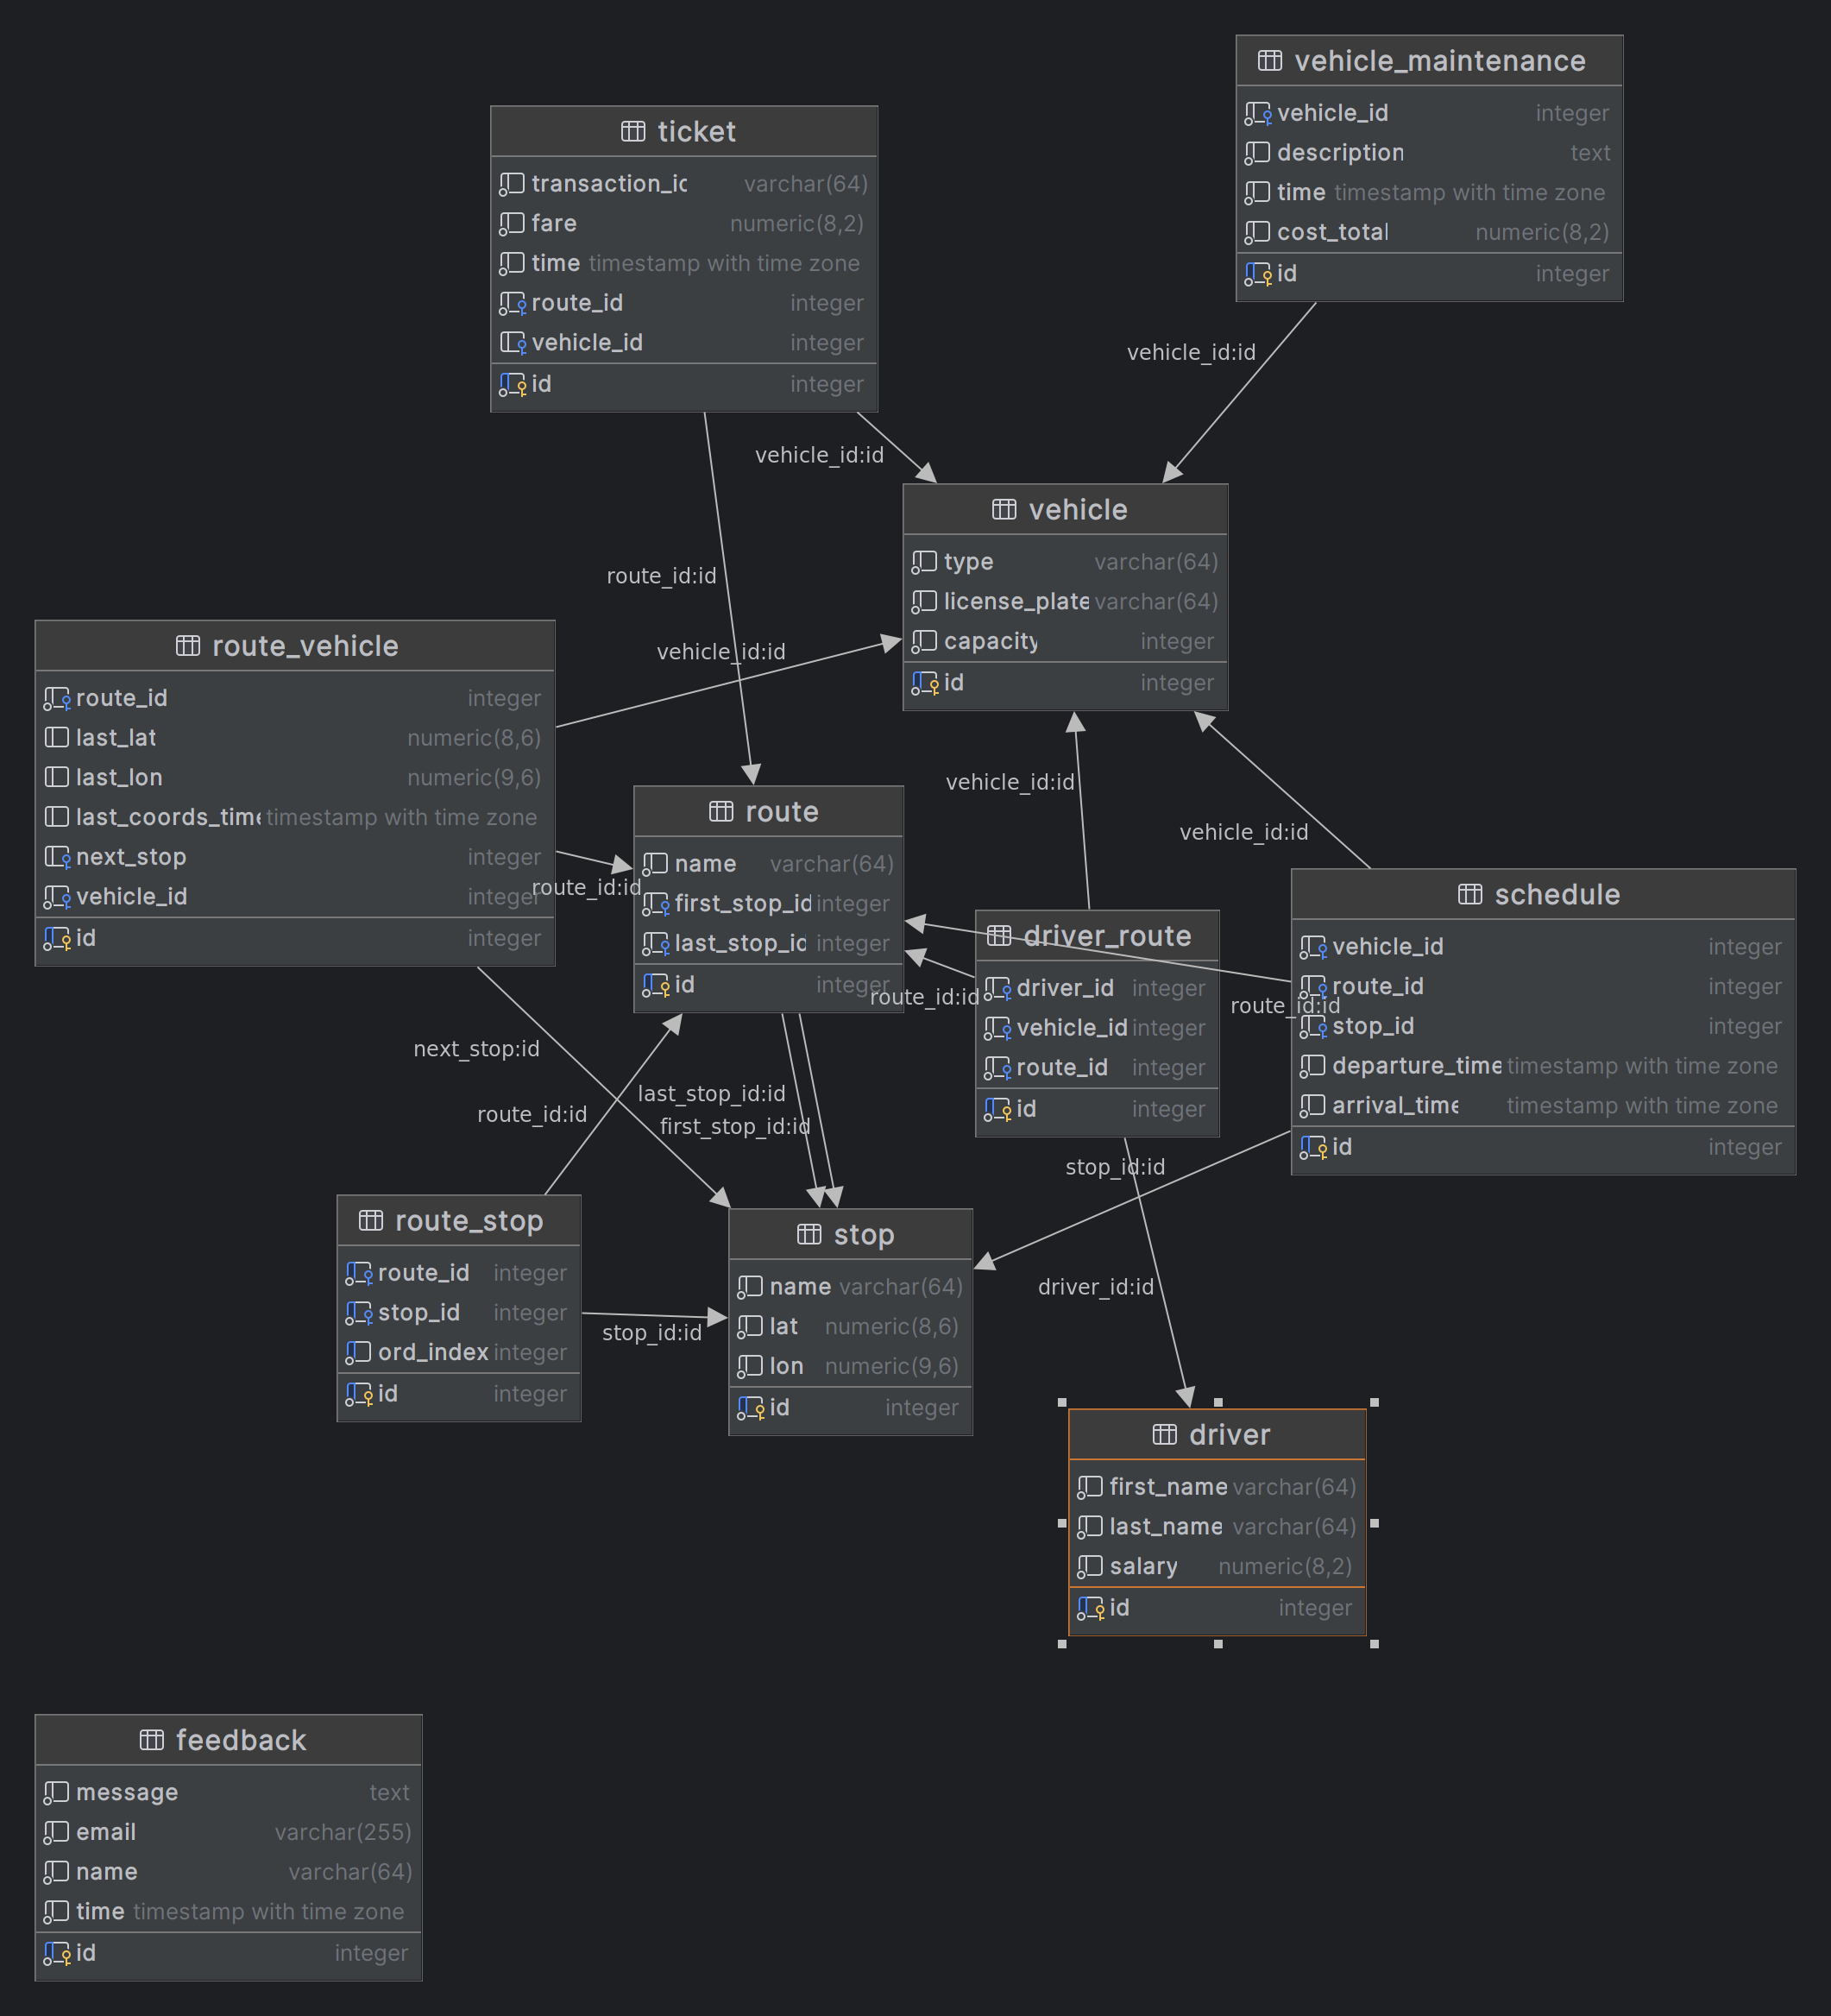
\includegraphics[scale=0.23]{6}
		\caption{Діаграма}
	\end{figure}
	
	
	\section*{Висновок}
	Під час виконання лабораторної роботи я розробив 5 запитів, що виконують вибірку із декількох таблиць предметної області. Врахував актуальність, форму представлення та можливі фільтри. Описав зміст запитів та корисні вхідні умови зафіксував текстом. Деякі запити зберіг як представлення (VIEW).
	Мої запити використовувють декілька операторів порівняння, базові функції обробки дати, рядків групування, агрегатні функції сортування, обмеження кількості.
	 
\end{normalsize}
\end{document}
